% 原书第 71—74 页；导言、5.1 节导言和 5.1.1 小节。
\chapter{与机器学习的联系（一）}
\label{ch:machine-learning-one}

如第 1 章所述，标准机器学习与统计学具有相同的基础：我们使用从某个未知底层分布独立同分布抽取的数据，尝试推断该分布的性质。相比之下，因果推断假定了一种更强的底层结构，其中包含有向的相依关系。这使得从数据中学习结构更加困难；但是，一旦学到了结构，就能作出新的论断，包括关于分布偏移和干预作用的论断。如果将机器学习看作推断某些超越纯粹统计关联的规律（或“自然定律”）的过程，那么因果性就发挥着至关重要的作用。本章将就此展开一些讨论，仅关注两个变量的情形。第 8 章会重新讨论这一主题，并考察多元情形。

\section{半监督学习}
\label{sec:ch05-semi-supervised-learning}

考虑一个回归任务，目标是根据 $d$ 维预测变量 $\mathbf{X}$ 来预测目标变量 $Y$。对于许多损失函数，只要知道条件分布 $P_{Y\mid\mathbf{X}}$，就足以解决问题。例如，回归函数
\[
 f^0(\mathbf{x})\coloneqq\EE[Y\mid\mathbf{X}=\mathbf{x}]
\]
能够使 $L_2$ 损失最小，即
\[
 f^0\in\mathop{\mathrm{arg\,min}}_{f:\RR^d\to\RR}
 \EE\bigl[(Y-f(\mathbf{X}))^2\bigr].
\]

在\textbf{监督学习（supervised learning）}中，我们获得从联合分布独立同分布抽取的 $n$ 个数据点：
\[
 ( \mathbf{X}_1,Y_1),\ldots,(\mathbf{X}_n,Y_n)
 \overset{\mathrm{iid}}{\sim}P_{\mathbf{X},Y}.
\]
因此，在 $L_2$ 损失下进行回归估计，就是利用联合分布中的 $n$ 个数据点来估计条件均值。然而，在（归纳式）\textbf{半监督学习（semi-supervised learning，SSL）}中，我们还会额外获得 $m$ 个无标签数据点
\[
 \mathbf{X}_{n+1},\ldots,\mathbf{X}_{n+m}
 \overset{\mathrm{iid}}{\sim}P_{\mathbf{X}}.
\]
我们希望，这些额外的数据点能够提供关于 $P_{\mathbf{X}}$ 的信息，而 $P_{\mathbf{X}}$ 又能告诉我们一些关于 $\EE[Y\mid\mathbf{X}]$ 的信息，或者更一般地，关于 $P_{Y\mid\mathbf{X}}$ 的信息。\footnote{这里仍用 $P_{Y\mid\mathbf{X}}$ 简记条件分布族 $(P_{Y\mid\mathbf{X}=\mathbf{x}})_{\mathbf{x}}$。}
许多半监督学习技术的基本假设，都涉及 $P_{\mathbf{X}}$ 与 $P_{Y\mid\mathbf{X}}$ 之间的联系，综述见 Chapelle et al.［2006］。例如，\textbf{聚类假设（cluster assumption）}规定，属于 $P_{\mathbf{X}}$ 同一个簇的点，其 $Y$ 值相同或相近。与之类似的\textbf{低密度分离假设（low-density separation assumption）}则规定，分类器的决策边界，即 $P(Y=1\mid\mathbf{X}=\mathbf{x})$ 穿过 $0.5$ 时对应的点 $\mathbf{x}$，应位于 $P_{\mathbf{X}}$ 密度较低的区域。\textbf{半监督光滑性假设（semi-supervised smoothness assumption）}规定，在 $P_{\mathbf{X}}$ 密度较高的区域，条件均值函数 $\mathbf{x}\mapsto\EE[Y\mid\mathbf{X}=\mathbf{x}]$ 应当是光滑的。

\subsection{半监督学习与因果方向}
\label{sec:ch05-ssl-causal-direction}

在最简单的情形下，因果图只包含两个变量，即原因和结果。此时，机器学习问题既可能沿因果方向展开，即根据原因预测结果；也可能沿\textbf{反因果方向（anticausal direction）}展开，即根据结果预测原因。实践工作者通常不关心给定学习问题背后的因果结构（见图 5.1）。但是，下面我们将说明，这种结构会对机器学习产生影响。

第 2.1 节提出，因果条件分布彼此独立，见原理 2.1 及其后的讨论。Schölkopf et al.［2012］认识到，这一原理对半监督学习具有直接含义。半监督学习依赖 $P_{\mathbf{X}}$ 与 $P_{Y\mid\mathbf{X}}$ 之间的联系，而该原理断言，$P_{\mathrm{cause}}$ 与 $P_{\mathrm{effect}\mid\mathrm{cause}}$ 不包含关于彼此的信息。因此可以推断：如果 $\mathbf{X}$ 对应原因，$Y$ 对应结果，即学习问题沿因果方向展开，那么半监督学习就不会起作用。在这种情况下，额外的 $\mathbf{x}$ 值只会增加我们对 $P_{\mathbf{X}}$ 的了解，但这些信息无助于预测，因为预测所需要的是关于独立对象 $P_{Y\mid\mathbf{X}}$ 的信息。反过来，如果 $\mathbf{X}$ 是结果、$Y$ 是原因，关于 $P_{\mathbf{X}}$ 的信息就可能告诉我们一些关于 $P_{Y\mid\mathbf{X}}$ 的信息。

一项综合分析半监督学习结果的研究支持了这一假设。在所有半监督学习有所帮助的情形中，学习问题或者沿反因果方向展开，或者存在混杂，或者其因果结构尚不明确，见图 5.2。

\begin{figure}[htbp]
\centering
\begin{tikzpicture}[causal,x=1cm,y=1cm,
 ch05amino/.style={circle,draw,fill=orange!35!red!25,minimum size=5.8mm,inner sep=1pt,font=\scriptsize},
 ch05bio/.style={font=\scriptsize,align=center}]
% 翻译原图的肽合成示意；核苷酸和氨基酸缩写按原图保留。
\begin{scope}[x=.82cm,y=.82cm]
\path[draw,fill=olive!50!gray]
 (2.1,1.6) .. controls (2.7,1.8) and (2.6,3.2) .. (3.8,3.2)
 .. controls (5.2,3.1) and (5.4,2.3) .. (5.3,1.2)
 .. controls (5.15,.1) and (4.4,.25) .. (2.9,.4)
 .. controls (2.4,.45) and (3.6,1.1) .. (2.1,1.6)--cycle;
\node[ch05bio] at (4.15,.86){核糖体};
\filldraw[fill=gray!50!green!15,draw=gray!80] (0,1.45) rectangle (8,1.72);
\foreach \x in {.08,.33,...,7.85}{
 \filldraw[fill=gray!50!green!15,draw=gray!80] (\x,1.72) rectangle ++(.1,.18);}
\node[font=\scriptsize,inner sep=1pt,fill=gray!50!green!15] at (3.5,1.58){U G G A A A G A U U U C};
\node[ch05bio] at (6.8,1.04){信使 RNA};
\foreach \x/\triplet in {3.15/U U U,4.1/C U A}{
 \path[draw,fill=yellow!85] (\x-.36,1.9)--(\x-.36,3.35)--(\x+.36,3.35)
 --(\x+.36,1.9)--(\x+.2,1.9)--(\x+.16,2.12)--(\x+.05,2.12)
 --(\x+.01,1.9)--(\x-.1,1.9)--(\x-.14,2.12)--(\x-.25,2.12)--(\x-.29,1.9)--cycle;
 \node[ch05bio,font=\tiny] at (\x,2.85){tRNA};
 \node[ch05bio,font=\tiny] at (\x,2.22){\triplet};
 \draw[thick] (\x,3.35)--(\x,4.1);}
\node[ch05amino] (ch05lys) at (3.15,4.1){Lys};
\node[ch05amino] (ch05asp) at (4.1,4.1){Asp};
\node[ch05amino] (ch05trp) at (2.25,4.38){Trp};
\node[ch05amino] (ch05aa2) at (1.57,4.95){};
\node[ch05amino] (ch05aa1) at (.93,5.51){};
\draw (ch05aa1)--(ch05aa2)--(ch05trp)--(ch05lys)--(ch05asp);
\node[ch05bio,anchor=west] at (1.8,5.55){正在延长的肽链};
\begin{scope}[shift={(1.1,3.55)},rotate=20]
\draw[thick] (0,.65)--(0,1.1);
\path[draw,fill=yellow!85] (-.35,-.8)--(-.35,.65)--(.35,.65)--(.35,-.8)
 --(.21,-.8)--(.17,-.57)--(.06,-.57)--(.02,-.8)--(-.09,-.8)--(-.13,-.57)--(-.24,-.57)--(-.28,-.8)--cycle;
\node[ch05bio,rotate=20] at (0,.05){tRNA};
\node[ch05bio,rotate=20] at (0,-.48){A C C};
\end{scope}
\node[ch05bio,anchor=east] at (.72,3.14){离开的\\空载 tRNA};
\draw[ed,very thick] (2.2,2.35)--(1.62,2.77);
\begin{scope}[shift={(6.3,3.48)},rotate=20]
\draw[thick] (0,.65)--(0,1.23);
\node[ch05amino] at (0,1.5){Phe};
\path[draw,fill=yellow!85] (-.35,-.8)--(-.35,.65)--(.35,.65)--(.35,-.8)
 --(.21,-.8)--(.17,-.57)--(.06,-.57)--(.02,-.8)--(-.09,-.8)--(-.13,-.57)--(-.24,-.57)--(-.28,-.8)--cycle;
\node[ch05bio,rotate=20] at (0,.05){tRNA};
\node[ch05bio,rotate=20] at (0,-.48){A A G};
\end{scope}
\node[ch05bio,anchor=west] at (6.65,4.13){进入的、结合\\氨基酸的 tRNA};
\draw[ed,very thick] (5.9,2.94)--(5.13,1.96);
\node[font=\small] at (4,-.05){肽合成};
\end{scope}
% 上：因果方向；下：反因果方向。绿色为预测，红色为因果关系。
\node[vtx] (ch05ax) at (8.6,2.8){$X$};
\node[vtx] (ch05ay) at (11.6,2.8){$Y$};
\node (ch05anx) at (8.6,1.3){$N_X$};
\node (ch05any) at (11.6,1.3){$N_Y$};
\draw[ed,red!85!black] (ch05ax)--node[below]{$\varphi$}(ch05ay);
\draw[ed,green!60!black,bend left=27] (ch05ax) to (ch05ay);
\draw[ed,blue!70!black] (ch05anx)--node[right]{$\mathrm{id}$}(ch05ax);
\draw[ed,red!85!black] (ch05any)--(ch05ay);
\node[inner sep=0pt] at (1.05,-1.7){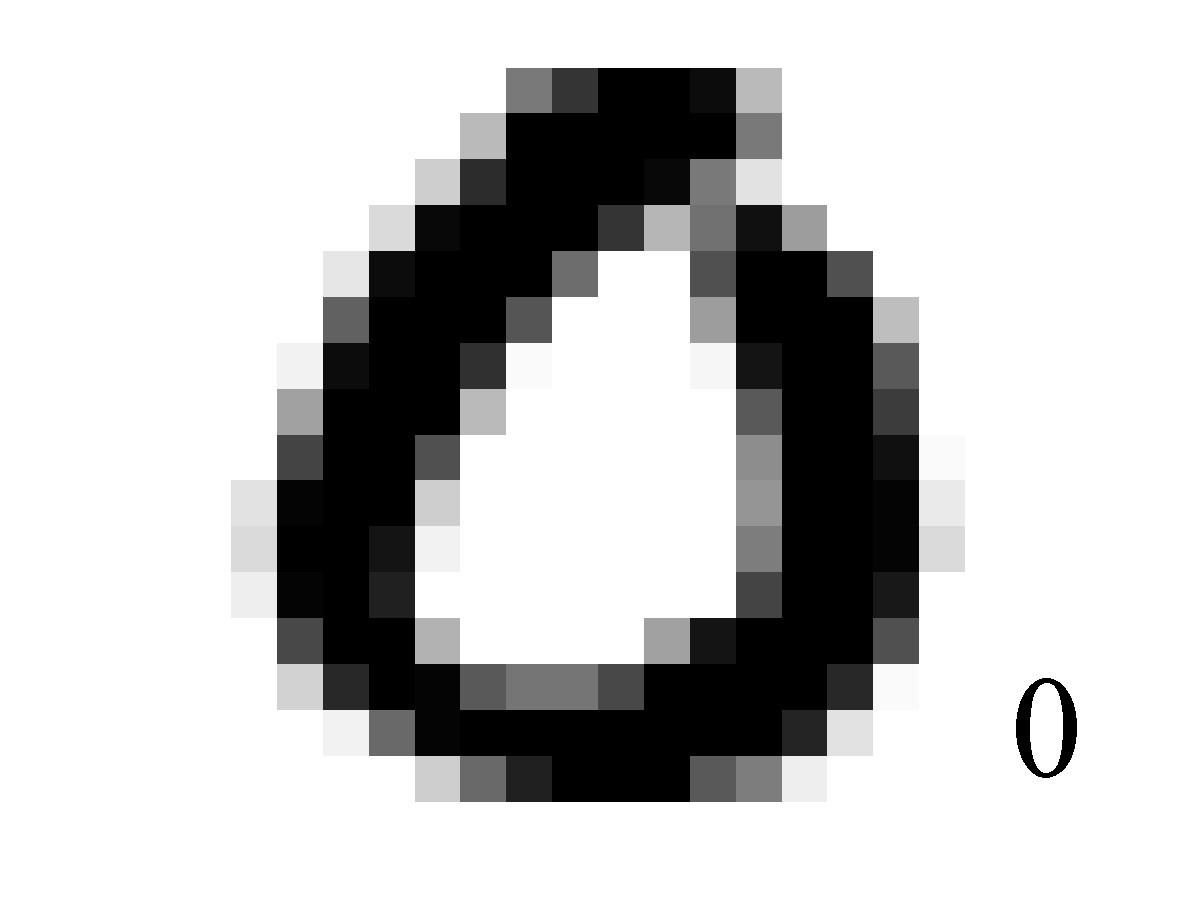
\includegraphics[width=2cm]{data/ch05_digit_0.jpg}};
\node[inner sep=0pt] at (3.35,-1.7){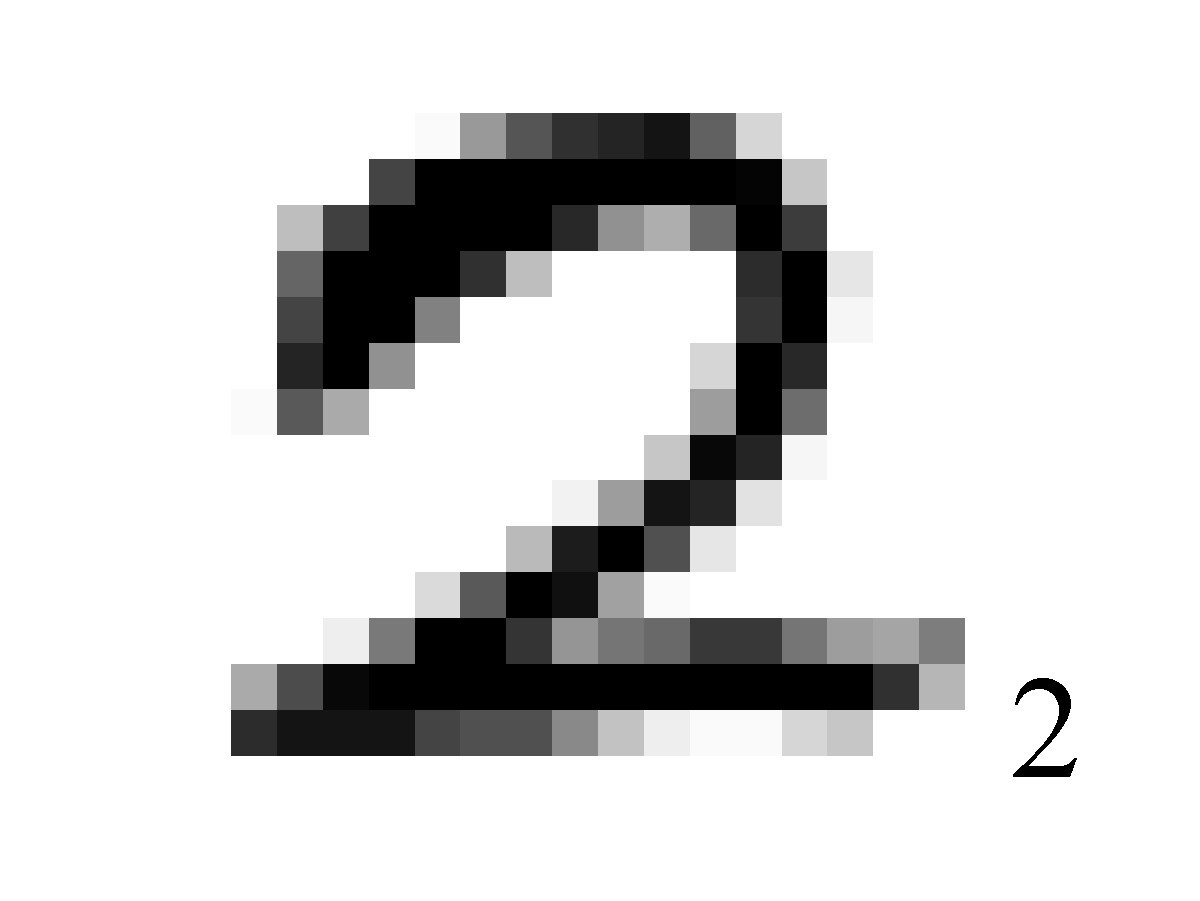
\includegraphics[width=2cm]{data/ch05_digit_2.jpg}};
\node[inner sep=0pt] at (5.65,-1.7){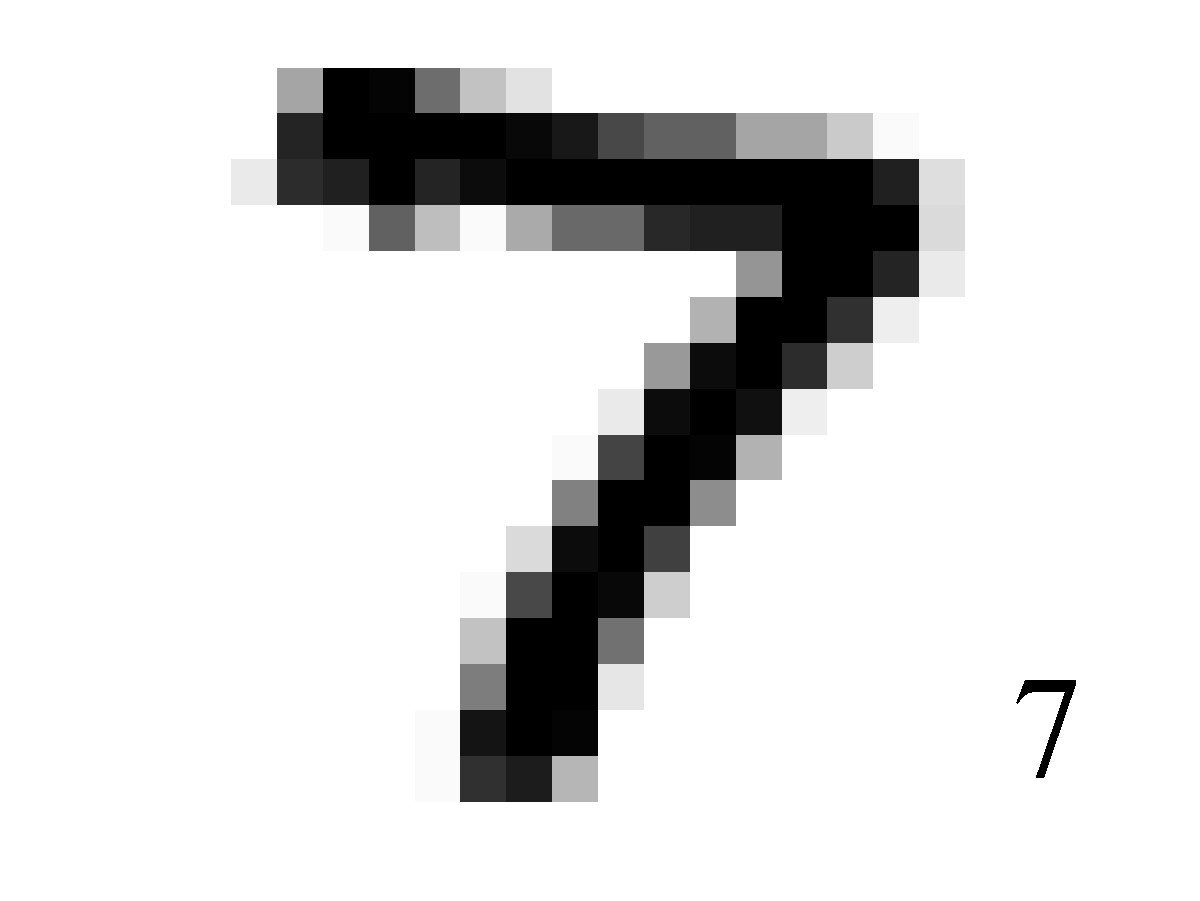
\includegraphics[width=2cm]{data/ch05_digit_7.jpg}};
\node[vtx] (ch05bx) at (8.6,-1.7){$X$};
\node[vtx] (ch05by) at (11.6,-1.7){$Y$};
\node (ch05bnx) at (8.6,-3.2){$N_X$};
\node (ch05bny) at (11.6,-3.2){$N_Y$};
\draw[ed,red!85!black] (ch05by)--node[below]{$\varphi$}(ch05bx);
\draw[ed,green!60!black,bend left=27] (ch05bx) to (ch05by);
\draw[ed,red!85!black] (ch05bnx)--(ch05bx);
\draw[ed,blue!70!black] (ch05bny)--node[right]{$\mathrm{id}$}(ch05by);
\end{tikzpicture}
\caption[因果与反因果预测任务]{上：称为核糖体的复杂机制 $\varphi$ 将 mRNA 信息 $X$ 翻译为蛋白质链 $Y$。\protect\footnotemark 根据 mRNA 预测蛋白质，是沿因果方向展开的学习问题；此时，预测方向（绿色箭头）与因果作用方向（红色箭头）一致。下：在手写数字识别中，我们试图根据书写者生成的图像 $X$，推断类别标签 $Y$，即书写者的意图。这是一个沿反因果方向展开的问题。}
\label{fig:ch05-learning-directions}
\end{figure}
\footnotetext{原肽合成图由用户“Boumphreyfr”提供：\url{https://commons.wikimedia.org/wiki/File:Peptide_syn.png}。许可为 CC BY-SA 3.0（\url{http://creativecommons.org/licenses/by-sa/3.0}）或 GFDL（\url{http://www.gnu.org/copyleft/fdl.html}）。本译稿以 TikZ 重绘其示意结构并翻译图中文字。}


在双射的确定性因果关系这一简化情景中（见第 4.1.7 节），Janzing and Schölkopf［2015］证明：只要 $P_{\mathrm{cause}}$ 与 $P_{\mathrm{effect}\mid\mathrm{cause}}$ 在式 (4.10) 的意义下相互独立，半监督学习就确实能在反因果方向上优于监督学习，而在因果方向上则不能。其思路是，半监督学习利用式 (4.11) 中的相依关系，构造更好的插值算法。Sgouritsa et al.［2015］利用“半监督学习只能在反因果方向上起作用”这一事实，开发了一种因果学习方法。

最后要注意，半监督学习还将某些形式的\textbf{无监督学习（unsupervised learning）}包含为特例，此时没有带标签的数据。例如，在聚类中，$Y$ 通常是表示簇编号的离散值。类似于上面的推理，我们可以认为，如果 $\mathbf{X}$ 是原因、$Y$ 是结果，聚类的表现应当不佳。不过，在许多对真实数据进行聚类的应用中，簇编号往往是特征的原因，而非其结果。

\begin{figure}[htbp]
\centering
\begingroup
\definecolor{ch05blue}{rgb}{.18155,.18994,.57328}
\definecolor{ch05green}{rgb}{.29407,.42391,.35215}
\definecolor{ch05red}{rgb}{.93042,.11090,.14145}
\begin{tikzpicture}[x=.43cm,y=.045cm]
\draw[line width=.4pt] (0,-78) rectangle (27,66);
\draw[gray,line width=.35pt] (0,0)--(27,0);
\foreach \v in {-60,-40,-20,0,20,40,60}{
 \draw (0,\v)--(-.25,\v) node[left,font=\scriptsize]{$\v$};}
\foreach \i/\name in {1/ba-sc,2/br-c,3/br-w,4/col,5/col.O,6/cr-a,7/cr-g,8/diab,9/he-c,10/he-h,11/he-s,12/hep,13/ion,14/iris,15/kr-kp,16/lab,17/lett,18/mush,19/seg,20/sick,21/son,22/splic,23/vehi,24/vote,25/vow,26/wave}{
 \draw (\i,-78)--(\i,-81);
 \node[rotate=90,anchor=east,font=\scriptsize] at (\i,-85){\name};}
\node[rotate=90,align=center,font=\small,text width=6.5cm] at (-3.25,-5)
 {使用自训练而非基础分类器时\\误差的相对降幅（\%）};
\begin{scope}
\clip (0,-77.852) rectangle (27,65.975);
% Coordinates recovered from printed vector markers, not original experimental data.
\fill[ch05blue] (3,18.62337) circle[x radius=.1611,y radius=1.5584];
\fill[ch05blue] (8,0.38961) circle[x radius=.1611,y radius=1.5584];
\fill[ch05blue] (12,8.55412) circle[x radius=.1611,y radius=1.5584];
\fill[ch05blue] (14,47.80952) circle[x radius=.1611,y radius=1.5584];
\fill[ch05blue] (16,51.29004) circle[x radius=.1611,y radius=1.5584];
\fill[ch05blue] (17,-45.14284) circle[x radius=.1611,y radius=1.5584];
\fill[ch05blue] (18,-10.76190) circle[x radius=.1611,y radius=1.5584];
\fill[ch05blue] (19,-72.52813) circle[x radius=.1611,y radius=1.5584];
\fill[ch05blue] (21,-20.14718) circle[x radius=.1611,y radius=1.5584];
\fill[ch05blue] (23,-23.48051) circle[x radius=.1611,y radius=1.5584];
\fill[ch05blue] (24,-13.15151) circle[x radius=.1611,y radius=1.5584];
\fill[ch05blue] (25,-20.45887) circle[x radius=.1611,y radius=1.5584];
\fill[ch05blue] (26,7.16018) circle[x radius=.1611,y radius=1.5584];
\fill[ch05blue] (3,11.43724) circle[x radius=.1611,y radius=1.5584];
\fill[ch05blue] (8,1.50650) circle[x radius=.1611,y radius=1.5584];
\fill[ch05blue] (12,7.40260) circle[x radius=.1611,y radius=1.5584];
\fill[ch05blue] (14,47.39394) circle[x radius=.1611,y radius=1.5584];
\fill[ch05blue] (16,38.71861) circle[x radius=.1611,y radius=1.5584];
\fill[ch05blue] (17,-4.47619) circle[x radius=.1611,y radius=1.5584];
\fill[ch05blue] (18,-17.64502) circle[x radius=.1611,y radius=1.5584];
\fill[ch05blue] (19,0.65801) circle[x radius=.1611,y radius=1.5584];
\fill[ch05blue] (21,-14.41557) circle[x radius=.1611,y radius=1.5584];
\fill[ch05blue] (23,-8.35497) circle[x radius=.1611,y radius=1.5584];
\fill[ch05blue] (24,-12.65801) circle[x radius=.1611,y radius=1.5584];
\fill[ch05blue] (25,-18.19046) circle[x radius=.1611,y radius=1.5584];
\fill[ch05blue] (26,7.61905) circle[x radius=.1611,y radius=1.5584];
\fill[ch05blue] (3,19.48052) circle[x radius=.1611,y radius=1.5584];
\fill[ch05blue] (8,1.55845) circle[x radius=.1611,y radius=1.5584];
\fill[ch05blue] (12,22.52814) circle[x radius=.1611,y radius=1.5584];
\fill[ch05blue] (14,51.30735) circle[x radius=.1611,y radius=1.5584];
\fill[ch05blue] (16,32.49350) circle[x radius=.1611,y radius=1.5584];
\fill[ch05blue] (17,-8.55411) circle[x radius=.1611,y radius=1.5584];
\fill[ch05blue] (18,-15.61904) circle[x radius=.1611,y radius=1.5584];
\fill[ch05blue] (19,-2.38095) circle[x radius=.1611,y radius=1.5584];
\fill[ch05blue] (21,6.19047) circle[x radius=.1611,y radius=1.5584];
\fill[ch05blue] (23,-5.51514) circle[x radius=.1611,y radius=1.5584];
\fill[ch05blue] (24,9.04762) circle[x radius=.1611,y radius=1.5584];
\fill[ch05blue] (25,-0.96104) circle[x radius=.1611,y radius=1.5584];
\fill[ch05blue] (26,6.64936) circle[x radius=.1611,y radius=1.5584];
\fill[ch05blue] (3,19.58441) circle[x radius=.1611,y radius=1.5584];
\fill[ch05blue] (8,6.03463) circle[x radius=.1611,y radius=1.5584];
\fill[ch05blue] (12,23.47186) circle[x radius=.1611,y radius=1.5584];
\fill[ch05blue] (14,60.64934) circle[x radius=.1611,y radius=1.5584];
\fill[ch05blue] (16,49.87013) circle[x radius=.1611,y radius=1.5584];
\fill[ch05blue] (17,-1.98267) circle[x radius=.1611,y radius=1.5584];
\fill[ch05blue] (18,-31.99133) circle[x radius=.1611,y radius=1.5584];
\fill[ch05blue] (19,-23.76622) circle[x radius=.1611,y radius=1.5584];
\fill[ch05blue] (21,14.88312) circle[x radius=.1611,y radius=1.5584];
\fill[ch05blue] (23,3.91343) circle[x radius=.1611,y radius=1.5584];
\fill[ch05blue] (24,1.87013) circle[x radius=.1611,y radius=1.5584];
\fill[ch05blue] (25,-4.07791) circle[x radius=.1611,y radius=1.5584];
\fill[ch05blue] (26,7.62770) circle[x radius=.1611,y radius=1.5584];
\fill[ch05blue] (3,16.73593) circle[x radius=.1611,y radius=1.5584];
\fill[ch05blue] (8,2.48485) circle[x radius=.1611,y radius=1.5584];
\fill[ch05blue] (12,19.68831) circle[x radius=.1611,y radius=1.5584];
\fill[ch05blue] (14,49.09090) circle[x radius=.1611,y radius=1.5584];
\fill[ch05blue] (16,45.29003) circle[x radius=.1611,y radius=1.5584];
\fill[ch05blue] (17,-1.33332) circle[x radius=.1611,y radius=1.5584];
\fill[ch05blue] (18,-3.22078) circle[x radius=.1611,y radius=1.5584];
\fill[ch05blue] (19,-1.66234) circle[x radius=.1611,y radius=1.5584];
\fill[ch05blue] (21,5.68832) circle[x radius=.1611,y radius=1.5584];
\fill[ch05blue] (23,1.07360) circle[x radius=.1611,y radius=1.5584];
\fill[ch05blue] (24,-3.16016) circle[x radius=.1611,y radius=1.5584];
\fill[ch05blue] (25,-5.99999) circle[x radius=.1611,y radius=1.5584];
\fill[ch05blue] (26,0.81386) circle[x radius=.1611,y radius=1.5584];
\fill[ch05blue] (3,22.06927) circle[x radius=.1611,y radius=1.5584];
\fill[ch05blue] (8,6.63204) circle[x radius=.1611,y radius=1.5584];
\fill[ch05blue] (12,1.76624) circle[x radius=.1611,y radius=1.5584];
\fill[ch05blue] (14,39.73160) circle[x radius=.1611,y radius=1.5584];
\fill[ch05blue] (16,18.19047) circle[x radius=.1611,y radius=1.5584];
\fill[ch05blue] (17,-14.08658) circle[x radius=.1611,y radius=1.5584];
\fill[ch05blue] (18,0.00001) circle[x radius=.1611,y radius=1.5584];
\fill[ch05blue] (19,-8.33766) circle[x radius=.1611,y radius=1.5584];
\fill[ch05blue] (21,-10.38095) circle[x radius=.1611,y radius=1.5584];
\fill[ch05blue] (23,-8.10389) circle[x radius=.1611,y radius=1.5584];
\fill[ch05blue] (24,-17.55843) circle[x radius=.1611,y radius=1.5584];
\fill[ch05blue] (25,-8.33766) circle[x radius=.1611,y radius=1.5584];
\fill[ch05blue] (26,6.86581) circle[x radius=.1611,y radius=1.5584];
\draw[ch05red,line width=.35pt] (0.7718,-63.29869)--(1.2282,-63.29869) (1,-65.50649)--(1,-61.09089) (0.8389,-64.85709)--(1.1611,-61.74029) (0.8389,-61.74029)--(1.1611,-64.85709);
\draw[ch05red,line width=.35pt] (14.7718,-63.68721)--(15.2282,-63.68721) (15,-65.89501)--(15,-61.47941) (14.8389,-65.24561)--(15.1611,-62.12881) (14.8389,-62.12881)--(15.1611,-65.24561);
\draw[ch05red,line width=.35pt] (21.7718,-72.39717)--(22.2282,-72.39717) (22,-74.60497)--(22,-70.18937) (21.8389,-73.95557)--(22.1611,-70.83877) (21.8389,-70.83877)--(22.1611,-73.95557);
\draw[ch05red,line width=.35pt] (0.7718,-41.34307)--(1.2282,-41.34307) (1,-43.55087)--(1,-39.13527) (0.8389,-42.90147)--(1.1611,-39.78467) (0.8389,-39.78467)--(1.1611,-42.90147);
\draw[ch05red,line width=.35pt] (14.7718,3.01407)--(15.2282,3.01407) (15,0.80627)--(15,5.22187) (14.8389,1.45567)--(15.1611,4.57247) (14.8389,4.57247)--(15.1611,1.45567);
\draw[ch05red,line width=.35pt] (21.7718,-72.84955)--(22.2282,-72.84955) (22,-75.05735)--(22,-70.64175) (21.8389,-74.40795)--(22.1611,-71.29115) (21.8389,-71.29115)--(22.1611,-74.40795);
\draw[ch05red,line width=.35pt] (0.7718,-25.42099)--(1.2282,-25.42099) (1,-27.62879)--(1,-23.21319) (0.8389,-26.97939)--(1.1611,-23.86259) (0.8389,-23.86259)--(1.1611,-26.97939);
\draw[ch05red,line width=.35pt] (14.7718,-89.12552)--(15.2282,-89.12552) (15,-91.33332)--(15,-86.91772) (14.8389,-90.68392)--(15.1611,-87.56712) (14.8389,-87.56712)--(15.1611,-90.68392);
\draw[ch05red,line width=.35pt] (21.7718,-6.19155)--(22.2282,-6.19155) (22,-8.39935)--(22,-3.98375) (21.8389,-7.74995)--(22.1611,-4.63315) (21.8389,-4.63315)--(22.1611,-7.74995);
\draw[ch05red,line width=.35pt] (0.7718,-0.86472)--(1.2282,-0.86472) (1,-3.07252)--(1,1.34308) (0.8389,-2.42312)--(1.1611,0.69368) (0.8389,0.69368)--(1.1611,-2.42312);
\draw[ch05red,line width=.35pt] (14.7718,-102.44911)--(15.2282,-102.44911) (15,-104.65691)--(15,-100.24131) (14.8389,-104.00751)--(15.1611,-100.89071) (14.8389,-100.89071)--(15.1611,-104.00751);
\draw[ch05red,line width=.35pt] (21.7718,-66.44262)--(22.2282,-66.44262) (22,-68.65042)--(22,-64.23482) (21.8389,-68.00102)--(22.1611,-64.88422) (21.8389,-64.88422)--(22.1611,-68.00102);
\draw[ch05red,line width=.35pt] (0.7718,-50.07683)--(1.2282,-50.07683) (1,-52.28463)--(1,-47.86903) (0.8389,-51.63523)--(1.1611,-48.51843) (0.8389,-48.51843)--(1.1611,-51.63523);
\draw[ch05red,line width=.35pt] (14.7718,-1.28895)--(15.2282,-1.28895) (15,-3.49675)--(15,0.91885) (14.8389,-2.84735)--(15.1611,0.26945) (14.8389,0.26945)--(15.1611,-2.84735);
\draw[ch05red,line width=.35pt] (21.7718,0.72836)--(22.2282,0.72836) (22,-1.47944)--(22,2.93616) (21.8389,-0.83004)--(22.1611,2.28676) (21.8389,2.28676)--(22.1611,-0.83004);
\draw[ch05red,line width=.35pt] (0.7718,-32.78787)--(1.2282,-32.78787) (1,-34.99567)--(1,-30.58007) (0.8389,-34.34627)--(1.1611,-31.22947) (0.8389,-31.22947)--(1.1611,-34.34627);
\draw[ch05red,line width=.35pt] (14.7718,-76.49457)--(15.2282,-76.49457) (15,-78.70237)--(15,-74.28677) (14.8389,-78.05297)--(15.1611,-74.93617) (14.8389,-74.93617)--(15.1611,-78.05297);
\draw[ch05red,line width=.35pt] (21.7718,-56.15691)--(22.2282,-56.15691) (22,-58.36471)--(22,-53.94911) (21.8389,-57.71531)--(22.1611,-54.59851) (21.8389,-54.59851)--(22.1611,-57.71531);
\draw[ch05green,line width=.35pt] (1.8389,-1.08220)--(2.1611,2.03460) (1.8389,2.03460)--(2.1611,-1.08220);
\draw[ch05green,line width=.35pt] (3.8389,-7.08221)--(4.1611,-3.96541) (3.8389,-3.96541)--(4.1611,-7.08221);
\draw[ch05green,line width=.35pt] (4.8389,-38.13848)--(5.1611,-35.02168) (4.8389,-35.02168)--(5.1611,-38.13848);
\draw[ch05green,line width=.35pt] (5.8389,-3.75753)--(6.1611,-0.64073) (5.8389,-0.64073)--(6.1611,-3.75753);
\draw[ch05green,line width=.35pt] (6.8389,-28.82246)--(7.1611,-25.70566) (6.8389,-25.70566)--(7.1611,-28.82246);
\draw[ch05green,line width=.35pt] (8.8389,13.21216)--(9.1611,16.32896) (8.8389,16.32896)--(9.1611,13.21216);
\draw[ch05green,line width=.35pt] (9.8389,8.72732)--(10.1611,11.84412) (9.8389,11.84412)--(10.1611,8.72732);
\draw[ch05green,line width=.35pt] (10.8389,9.16887)--(11.1611,12.28567) (10.8389,12.28567)--(11.1611,9.16887);
\draw[ch05green,line width=.35pt] (12.8389,4.96108)--(13.1611,8.07788) (12.8389,8.07788)--(13.1611,4.96108);
\draw[ch05green,line width=.35pt] (19.8389,-47.34193)--(20.1611,-44.22513) (19.8389,-44.22513)--(20.1611,-47.34193);
\draw[ch05green,line width=.35pt] (1.8389,-14.52809)--(2.1611,-11.41129) (1.8389,-11.41129)--(2.1611,-14.52809);
\draw[ch05green,line width=.35pt] (3.8389,17.79225)--(4.1611,20.90905) (3.8389,20.90905)--(4.1611,17.79225);
\draw[ch05green,line width=.35pt] (4.8389,-28.92635)--(5.1611,-25.80955) (4.8389,-25.80955)--(5.1611,-28.92635);
\draw[ch05green,line width=.35pt] (5.8389,-7.05623)--(6.1611,-3.93943) (5.8389,-3.93943)--(6.1611,-7.05623);
\draw[ch05green,line width=.35pt] (6.8389,-8.64065)--(7.1611,-5.52385) (6.8389,-5.52385)--(7.1611,-8.64065);
\draw[ch05green,line width=.35pt] (8.8389,3.35069)--(9.1611,6.46749) (8.8389,6.46749)--(9.1611,3.35069);
\draw[ch05green,line width=.35pt] (9.8389,1.19485)--(10.1611,4.31165) (9.8389,4.31165)--(10.1611,1.19485);
\draw[ch05green,line width=.35pt] (10.8389,-4.25969)--(11.1611,-1.14289) (10.8389,-1.14289)--(11.1611,-4.25969);
\draw[ch05green,line width=.35pt] (12.8389,-2.85710)--(13.1611,0.25970) (12.8389,0.25970)--(13.1611,-2.85710);
\draw[ch05green,line width=.35pt] (19.8389,-36.24237)--(20.1611,-33.12557) (19.8389,-33.12557)--(20.1611,-36.24237);
\draw[ch05green,line width=.35pt] (1.8389,-2.32896)--(2.1611,0.78784) (1.8389,0.78784)--(2.1611,-2.32896);
\draw[ch05green,line width=.35pt] (3.8389,22.92645)--(4.1611,26.04325) (3.8389,26.04325)--(4.1611,22.92645);
\draw[ch05green,line width=.35pt] (4.8389,-11.75753)--(5.1611,-8.64073) (4.8389,-8.64073)--(5.1611,-11.75753);
\draw[ch05green,line width=.35pt] (5.8389,14.83121)--(6.1611,17.94801) (5.8389,17.94801)--(6.1611,14.83121);
\draw[ch05green,line width=.35pt] (6.8389,-10.96964)--(7.1611,-7.85284) (6.8389,-7.85284)--(7.1611,-10.96964);
\draw[ch05green,line width=.35pt] (8.8389,30.85718)--(9.1611,33.97398) (8.8389,33.97398)--(9.1611,30.85718);
\draw[ch05green,line width=.35pt] (9.8389,31.74030)--(10.1611,34.85710) (9.8389,34.85710)--(10.1611,31.74030);
\draw[ch05green,line width=.35pt] (10.8389,14.66671)--(11.1611,17.78351) (10.8389,17.78351)--(11.1611,14.66671);
\draw[ch05green,line width=.35pt] (12.8389,10.87450)--(13.1611,13.99130) (12.8389,13.99130)--(13.1611,10.87450);
\draw[ch05green,line width=.35pt] (19.8389,-64.46748)--(20.1611,-61.35068) (19.8389,-61.35068)--(20.1611,-64.46748);
\draw[ch05green,line width=.35pt] (1.8389,3.98273)--(2.1611,7.09953) (1.8389,7.09953)--(2.1611,3.98273);
\draw[ch05green,line width=.35pt] (3.8389,14.88316)--(4.1611,17.99996) (3.8389,17.99996)--(4.1611,14.88316);
\draw[ch05green,line width=.35pt] (4.8389,-2.80516)--(5.1611,0.31164) (4.8389,0.31164)--(5.1611,-2.80516);
\draw[ch05green,line width=.35pt] (5.8389,2.96108)--(6.1611,6.07788) (5.8389,6.07788)--(6.1611,2.96108);
\draw[ch05green,line width=.35pt] (6.8389,-5.42853)--(7.1611,-2.31173) (6.8389,-2.31173)--(7.1611,-5.42853);
\draw[ch05green,line width=.35pt] (8.8389,27.23814)--(9.1611,30.35494) (8.8389,30.35494)--(9.1611,27.23814);
\draw[ch05green,line width=.35pt] (9.8389,21.23813)--(10.1611,24.35493) (9.8389,24.35493)--(10.1611,21.23813);
\draw[ch05green,line width=.35pt] (10.8389,28.64074)--(11.1611,31.75754) (10.8389,31.75754)--(11.1611,28.64074);
\draw[ch05green,line width=.35pt] (12.8389,6.14723)--(13.1611,9.26403) (12.8389,9.26403)--(13.1611,6.14723);
\draw[ch05green,line width=.35pt] (19.8389,-88.30297)--(20.1611,-85.18617) (19.8389,-85.18617)--(20.1611,-88.30297);
\draw[ch05green,line width=.35pt] (1.8389,-2.75320)--(2.1611,0.36360) (1.8389,0.36360)--(2.1611,-2.75320);
\draw[ch05green,line width=.35pt] (3.8389,14.33771)--(4.1611,17.45451) (3.8389,17.45451)--(4.1611,14.33771);
\draw[ch05green,line width=.35pt] (4.8389,-17.21207)--(5.1611,-14.09527) (4.8389,-14.09527)--(5.1611,-17.21207);
\draw[ch05green,line width=.35pt] (5.8389,0.33771)--(6.1611,3.45451) (5.8389,3.45451)--(6.1611,0.33771);
\draw[ch05green,line width=.35pt] (6.8389,-6.95233)--(7.1611,-3.83553) (6.8389,-3.83553)--(7.1611,-6.95233);
\draw[ch05green,line width=.35pt] (8.8389,14.07796)--(9.1611,17.19476) (8.8389,17.19476)--(9.1611,14.07796);
\draw[ch05green,line width=.35pt] (9.8389,11.38532)--(10.1611,14.50212) (9.8389,14.50212)--(10.1611,11.38532);
\draw[ch05green,line width=.35pt] (10.8389,10.16455)--(11.1611,13.28135) (10.8389,13.28135)--(11.1611,10.16455);
\draw[ch05green,line width=.35pt] (12.8389,6.55416)--(13.1611,9.67096) (12.8389,9.67096)--(13.1611,6.55416);
\draw[ch05green,line width=.35pt] (19.8389,-4.25103)--(20.1611,-1.13423) (19.8389,-1.13423)--(20.1611,-4.25103);
\draw[ch05green,line width=.35pt] (1.8389,-3.16013)--(2.1611,-0.04333) (1.8389,-0.04333)--(2.1611,-3.16013);
\draw[ch05green,line width=.35pt] (3.8389,8.24246)--(4.1611,11.35926) (3.8389,11.35926)--(4.1611,8.24246);
\draw[ch05green,line width=.35pt] (4.8389,-30.74454)--(5.1611,-27.62774) (4.8389,-27.62774)--(5.1611,-30.74454);
\draw[ch05green,line width=.35pt] (5.8389,7.07364)--(6.1611,10.19044) (5.8389,10.19044)--(6.1611,7.07364);
\draw[ch05green,line width=.35pt] (6.8389,-14.73588)--(7.1611,-11.61908) (6.8389,-11.61908)--(7.1611,-14.73588);
\draw[ch05green,line width=.35pt] (8.8389,24.98705)--(9.1611,28.10385) (8.8389,28.10385)--(9.1611,24.98705);
\draw[ch05green,line width=.35pt] (9.8389,22.90914)--(10.1611,26.02594) (9.8389,26.02594)--(10.1611,22.90914);
\draw[ch05green,line width=.35pt] (10.8389,6.80524)--(11.1611,9.92204) (10.8389,9.92204)--(11.1611,6.80524);
\draw[ch05green,line width=.35pt] (12.8389,26.47623)--(13.1611,29.59303) (12.8389,29.59303)--(13.1611,26.47623);
\draw[ch05green,line width=.35pt] (19.8389,-73.93934)--(20.1611,-70.82254) (19.8389,-70.82254)--(20.1611,-73.93934);

\end{scope}
\filldraw[fill=white,draw=black,line width=.35pt] (17.6,63)--(26.7,63)--(26.7,30)--(17.6,30)--cycle;
\fill[ch05blue] (18.3,56) circle[x radius=.16,y radius=1.55];
\node[anchor=west,font=\scriptsize] at (19,56){反因果／存在混杂};
\node[ch05red,font=\small] at (18.3,46.5){$\ast$};
\node[anchor=west,font=\scriptsize] at (19,46.5){因果};
\node[ch05green,font=\small] at (18.3,37){$\times$};
\node[anchor=west,font=\scriptsize] at (19,37){不明确};
\end{tikzpicture}
\endgroup
\caption{半监督学习的收益取决于因果结构。每一列点对应 UCI 数据仓库中的一个基准数据集，展示六种不同的基础分类器（base classifier）加入自训练（self-training）后的表现。自训练是一种通用的半监督学习方法。表现以误差相对于基础分类器的百分比降幅衡量，即 $(\operatorname{error}(\mathrm{base})-\operatorname{error}(\mathrm{self\text{-}train}))/\operatorname{error}(\mathrm{base})$。总体而言，自训练无助于因果数据集，但对部分反因果或存在混杂的数据集有所帮助［引自 Schölkopf et al., 2012］。}
\label{fig:ch05-ssl-benchmarks}
\end{figure}


虽然图 5.2 中的经验结果令人期待，但“半监督学习在因果方向上不起作用”这一说法仍需更精确地表述；这里始终假定原因与机制独立，参见原理 2.1。下一小节将作出更精确的说明。对半监督学习和\textbf{协变量偏移（covariate shift）}感兴趣的读者，可以关注这部分内容；其他读者初读时可以跳过。
\FloatBarrier
